



    
% !TeX spellcheck = de_DE
% !TeX encoding = UTF-8
\documentclass{article}
% \usepackage{ngerman}

    
    
    \usepackage[T1]{fontenc}
    % Nicer default font (+ math font) than Computer Modern for most use cases
    \usepackage{mathpazo}

    % Basic figure setup, for now with no caption control since it's done
    % automatically by Pandoc (which extracts ![](path) syntax from Markdown).
    \usepackage{graphicx}
    % We will generate all images so they have a width \maxwidth. This means
    % that they will get their normal width if they fit onto the page, but
    % are scaled down if they would overflow the margins.
    \makeatletter
    \def\maxwidth{\ifdim\Gin@nat@width>\linewidth\linewidth
    \else\Gin@nat@width\fi}
    \makeatother
    \let\Oldincludegraphics\includegraphics
    % Set max figure width to be 80% of text width, for now hardcoded.
    \renewcommand{\includegraphics}[1]{\Oldincludegraphics[width=.8\maxwidth]{#1}}
    % Ensure that by default, figures have no caption (until we provide a
    % proper Figure object with a Caption API and a way to capture that
    % in the conversion process - todo).
    \usepackage{caption}
    \DeclareCaptionLabelFormat{nolabel}{}
    \captionsetup{labelformat=nolabel}

    \usepackage{adjustbox} % Used to constrain images to a maximum size 
    \usepackage{xcolor} % Allow colors to be defined
    \usepackage{enumerate} % Needed for markdown enumerations to work
    \usepackage{geometry} % Used to adjust the document margins
    \usepackage{amsmath} % Equations
    \usepackage{amssymb} % Equations
    \usepackage{textcomp} % defines textquotesingle
    % Hack from http://tex.stackexchange.com/a/47451/13684:
    \AtBeginDocument{%
        \def\PYZsq{\textquotesingle}% Upright quotes in Pygmentized code
    }
    \usepackage{upquote} % Upright quotes for verbatim code
    \usepackage{eurosym} % defines \euro
    \usepackage[mathletters]{ucs} % Extended unicode (utf-8) support
    \usepackage[utf8x]{inputenc} % Allow utf-8 characters in the tex document
    \usepackage{fancyvrb} % verbatim replacement that allows latex
    \usepackage{grffile} % extends the file name processing of package graphics 
                         % to support a larger range 
    % The hyperref package gives us a pdf with properly built
    % internal navigation ('pdf bookmarks' for the table of contents,
    % internal cross-reference links, web links for URLs, etc.)
    \usepackage{hyperref}
    \usepackage{longtable} % longtable support required by pandoc >1.10
    \usepackage{booktabs}  % table support for pandoc > 1.12.2
    \usepackage[inline]{enumitem} % IRkernel/repr support (it uses the enumerate* environment)
    \usepackage[normalem]{ulem} % ulem is needed to support strikethroughs (\sout)
                                % normalem makes italics be italics, not underlines
    

    
    
    % Colors for the hyperref package
    \definecolor{urlcolor}{rgb}{0,.145,.698}
    \definecolor{linkcolor}{rgb}{.71,0.21,0.01}
    \definecolor{citecolor}{rgb}{.12,.54,.11}

    % ANSI colors
    \definecolor{ansi-black}{HTML}{3E424D}
    \definecolor{ansi-black-intense}{HTML}{282C36}
    \definecolor{ansi-red}{HTML}{E75C58}
    \definecolor{ansi-red-intense}{HTML}{B22B31}
    \definecolor{ansi-green}{HTML}{00A250}
    \definecolor{ansi-green-intense}{HTML}{007427}
    \definecolor{ansi-yellow}{HTML}{DDB62B}
    \definecolor{ansi-yellow-intense}{HTML}{B27D12}
    \definecolor{ansi-blue}{HTML}{208FFB}
    \definecolor{ansi-blue-intense}{HTML}{0065CA}
    \definecolor{ansi-magenta}{HTML}{D160C4}
    \definecolor{ansi-magenta-intense}{HTML}{A03196}
    \definecolor{ansi-cyan}{HTML}{60C6C8}
    \definecolor{ansi-cyan-intense}{HTML}{258F8F}
    \definecolor{ansi-white}{HTML}{C5C1B4}
    \definecolor{ansi-white-intense}{HTML}{A1A6B2}

    % commands and environments needed by pandoc snippets
    % extracted from the output of `pandoc -s`
    \providecommand{\tightlist}{%
      \setlength{\itemsep}{0pt}\setlength{\parskip}{0pt}}
    \DefineVerbatimEnvironment{Highlighting}{Verbatim}{commandchars=\\\{\}}
    % Add ',fontsize=\small' for more characters per line
    \newenvironment{Shaded}{}{}
    \newcommand{\KeywordTok}[1]{\textcolor[rgb]{0.00,0.44,0.13}{\textbf{{#1}}}}
    \newcommand{\DataTypeTok}[1]{\textcolor[rgb]{0.56,0.13,0.00}{{#1}}}
    \newcommand{\DecValTok}[1]{\textcolor[rgb]{0.25,0.63,0.44}{{#1}}}
    \newcommand{\BaseNTok}[1]{\textcolor[rgb]{0.25,0.63,0.44}{{#1}}}
    \newcommand{\FloatTok}[1]{\textcolor[rgb]{0.25,0.63,0.44}{{#1}}}
    \newcommand{\CharTok}[1]{\textcolor[rgb]{0.25,0.44,0.63}{{#1}}}
    \newcommand{\StringTok}[1]{\textcolor[rgb]{0.25,0.44,0.63}{{#1}}}
    \newcommand{\CommentTok}[1]{\textcolor[rgb]{0.38,0.63,0.69}{\textit{{#1}}}}
    \newcommand{\OtherTok}[1]{\textcolor[rgb]{0.00,0.44,0.13}{{#1}}}
    \newcommand{\AlertTok}[1]{\textcolor[rgb]{1.00,0.00,0.00}{\textbf{{#1}}}}
    \newcommand{\FunctionTok}[1]{\textcolor[rgb]{0.02,0.16,0.49}{{#1}}}
    \newcommand{\RegionMarkerTok}[1]{{#1}}
    \newcommand{\ErrorTok}[1]{\textcolor[rgb]{1.00,0.00,0.00}{\textbf{{#1}}}}
    \newcommand{\NormalTok}[1]{{#1}}
    
    % Additional commands for more recent versions of Pandoc
    \newcommand{\ConstantTok}[1]{\textcolor[rgb]{0.53,0.00,0.00}{{#1}}}
    \newcommand{\SpecialCharTok}[1]{\textcolor[rgb]{0.25,0.44,0.63}{{#1}}}
    \newcommand{\VerbatimStringTok}[1]{\textcolor[rgb]{0.25,0.44,0.63}{{#1}}}
    \newcommand{\SpecialStringTok}[1]{\textcolor[rgb]{0.73,0.40,0.53}{{#1}}}
    \newcommand{\ImportTok}[1]{{#1}}
    \newcommand{\DocumentationTok}[1]{\textcolor[rgb]{0.73,0.13,0.13}{\textit{{#1}}}}
    \newcommand{\AnnotationTok}[1]{\textcolor[rgb]{0.38,0.63,0.69}{\textbf{\textit{{#1}}}}}
    \newcommand{\CommentVarTok}[1]{\textcolor[rgb]{0.38,0.63,0.69}{\textbf{\textit{{#1}}}}}
    \newcommand{\VariableTok}[1]{\textcolor[rgb]{0.10,0.09,0.49}{{#1}}}
    \newcommand{\ControlFlowTok}[1]{\textcolor[rgb]{0.00,0.44,0.13}{\textbf{{#1}}}}
    \newcommand{\OperatorTok}[1]{\textcolor[rgb]{0.40,0.40,0.40}{{#1}}}
    \newcommand{\BuiltInTok}[1]{{#1}}
    \newcommand{\ExtensionTok}[1]{{#1}}
    \newcommand{\PreprocessorTok}[1]{\textcolor[rgb]{0.74,0.48,0.00}{{#1}}}
    \newcommand{\AttributeTok}[1]{\textcolor[rgb]{0.49,0.56,0.16}{{#1}}}
    \newcommand{\InformationTok}[1]{\textcolor[rgb]{0.38,0.63,0.69}{\textbf{\textit{{#1}}}}}
    \newcommand{\WarningTok}[1]{\textcolor[rgb]{0.38,0.63,0.69}{\textbf{\textit{{#1}}}}}
    
    
    % Define a nice break command that doesn't care if a line doesn't already
    % exist.
    \def\br{\hspace*{\fill} \\* }
    % Math Jax compatability definitions
    \def\gt{>}
    \def\lt{<}
    % Document parameters
    \title{VariableTransmissions}
    
    
    

    % Pygments definitions
    
\makeatletter
\def\PY@reset{\let\PY@it=\relax \let\PY@bf=\relax%
    \let\PY@ul=\relax \let\PY@tc=\relax%
    \let\PY@bc=\relax \let\PY@ff=\relax}
\def\PY@tok#1{\csname PY@tok@#1\endcsname}
\def\PY@toks#1+{\ifx\relax#1\empty\else%
    \PY@tok{#1}\expandafter\PY@toks\fi}
\def\PY@do#1{\PY@bc{\PY@tc{\PY@ul{%
    \PY@it{\PY@bf{\PY@ff{#1}}}}}}}
\def\PY#1#2{\PY@reset\PY@toks#1+\relax+\PY@do{#2}}

\expandafter\def\csname PY@tok@gd\endcsname{\def\PY@tc##1{\textcolor[rgb]{0.63,0.00,0.00}{##1}}}
\expandafter\def\csname PY@tok@gu\endcsname{\let\PY@bf=\textbf\def\PY@tc##1{\textcolor[rgb]{0.50,0.00,0.50}{##1}}}
\expandafter\def\csname PY@tok@gt\endcsname{\def\PY@tc##1{\textcolor[rgb]{0.00,0.27,0.87}{##1}}}
\expandafter\def\csname PY@tok@gs\endcsname{\let\PY@bf=\textbf}
\expandafter\def\csname PY@tok@gr\endcsname{\def\PY@tc##1{\textcolor[rgb]{1.00,0.00,0.00}{##1}}}
\expandafter\def\csname PY@tok@cm\endcsname{\let\PY@it=\textit\def\PY@tc##1{\textcolor[rgb]{0.25,0.50,0.50}{##1}}}
\expandafter\def\csname PY@tok@vg\endcsname{\def\PY@tc##1{\textcolor[rgb]{0.10,0.09,0.49}{##1}}}
\expandafter\def\csname PY@tok@vi\endcsname{\def\PY@tc##1{\textcolor[rgb]{0.10,0.09,0.49}{##1}}}
\expandafter\def\csname PY@tok@mh\endcsname{\def\PY@tc##1{\textcolor[rgb]{0.40,0.40,0.40}{##1}}}
\expandafter\def\csname PY@tok@cs\endcsname{\let\PY@it=\textit\def\PY@tc##1{\textcolor[rgb]{0.25,0.50,0.50}{##1}}}
\expandafter\def\csname PY@tok@ge\endcsname{\let\PY@it=\textit}
\expandafter\def\csname PY@tok@vc\endcsname{\def\PY@tc##1{\textcolor[rgb]{0.10,0.09,0.49}{##1}}}
\expandafter\def\csname PY@tok@il\endcsname{\def\PY@tc##1{\textcolor[rgb]{0.40,0.40,0.40}{##1}}}
\expandafter\def\csname PY@tok@go\endcsname{\def\PY@tc##1{\textcolor[rgb]{0.53,0.53,0.53}{##1}}}
\expandafter\def\csname PY@tok@cp\endcsname{\def\PY@tc##1{\textcolor[rgb]{0.74,0.48,0.00}{##1}}}
\expandafter\def\csname PY@tok@gi\endcsname{\def\PY@tc##1{\textcolor[rgb]{0.00,0.63,0.00}{##1}}}
\expandafter\def\csname PY@tok@gh\endcsname{\let\PY@bf=\textbf\def\PY@tc##1{\textcolor[rgb]{0.00,0.00,0.50}{##1}}}
\expandafter\def\csname PY@tok@ni\endcsname{\let\PY@bf=\textbf\def\PY@tc##1{\textcolor[rgb]{0.60,0.60,0.60}{##1}}}
\expandafter\def\csname PY@tok@nl\endcsname{\def\PY@tc##1{\textcolor[rgb]{0.63,0.63,0.00}{##1}}}
\expandafter\def\csname PY@tok@nn\endcsname{\let\PY@bf=\textbf\def\PY@tc##1{\textcolor[rgb]{0.00,0.00,1.00}{##1}}}
\expandafter\def\csname PY@tok@no\endcsname{\def\PY@tc##1{\textcolor[rgb]{0.53,0.00,0.00}{##1}}}
\expandafter\def\csname PY@tok@na\endcsname{\def\PY@tc##1{\textcolor[rgb]{0.49,0.56,0.16}{##1}}}
\expandafter\def\csname PY@tok@nb\endcsname{\def\PY@tc##1{\textcolor[rgb]{0.00,0.50,0.00}{##1}}}
\expandafter\def\csname PY@tok@nc\endcsname{\let\PY@bf=\textbf\def\PY@tc##1{\textcolor[rgb]{0.00,0.00,1.00}{##1}}}
\expandafter\def\csname PY@tok@nd\endcsname{\def\PY@tc##1{\textcolor[rgb]{0.67,0.13,1.00}{##1}}}
\expandafter\def\csname PY@tok@ne\endcsname{\let\PY@bf=\textbf\def\PY@tc##1{\textcolor[rgb]{0.82,0.25,0.23}{##1}}}
\expandafter\def\csname PY@tok@nf\endcsname{\def\PY@tc##1{\textcolor[rgb]{0.00,0.00,1.00}{##1}}}
\expandafter\def\csname PY@tok@si\endcsname{\let\PY@bf=\textbf\def\PY@tc##1{\textcolor[rgb]{0.73,0.40,0.53}{##1}}}
\expandafter\def\csname PY@tok@s2\endcsname{\def\PY@tc##1{\textcolor[rgb]{0.73,0.13,0.13}{##1}}}
\expandafter\def\csname PY@tok@nt\endcsname{\let\PY@bf=\textbf\def\PY@tc##1{\textcolor[rgb]{0.00,0.50,0.00}{##1}}}
\expandafter\def\csname PY@tok@nv\endcsname{\def\PY@tc##1{\textcolor[rgb]{0.10,0.09,0.49}{##1}}}
\expandafter\def\csname PY@tok@s1\endcsname{\def\PY@tc##1{\textcolor[rgb]{0.73,0.13,0.13}{##1}}}
\expandafter\def\csname PY@tok@ch\endcsname{\let\PY@it=\textit\def\PY@tc##1{\textcolor[rgb]{0.25,0.50,0.50}{##1}}}
\expandafter\def\csname PY@tok@m\endcsname{\def\PY@tc##1{\textcolor[rgb]{0.40,0.40,0.40}{##1}}}
\expandafter\def\csname PY@tok@gp\endcsname{\let\PY@bf=\textbf\def\PY@tc##1{\textcolor[rgb]{0.00,0.00,0.50}{##1}}}
\expandafter\def\csname PY@tok@sh\endcsname{\def\PY@tc##1{\textcolor[rgb]{0.73,0.13,0.13}{##1}}}
\expandafter\def\csname PY@tok@ow\endcsname{\let\PY@bf=\textbf\def\PY@tc##1{\textcolor[rgb]{0.67,0.13,1.00}{##1}}}
\expandafter\def\csname PY@tok@sx\endcsname{\def\PY@tc##1{\textcolor[rgb]{0.00,0.50,0.00}{##1}}}
\expandafter\def\csname PY@tok@bp\endcsname{\def\PY@tc##1{\textcolor[rgb]{0.00,0.50,0.00}{##1}}}
\expandafter\def\csname PY@tok@c1\endcsname{\let\PY@it=\textit\def\PY@tc##1{\textcolor[rgb]{0.25,0.50,0.50}{##1}}}
\expandafter\def\csname PY@tok@o\endcsname{\def\PY@tc##1{\textcolor[rgb]{0.40,0.40,0.40}{##1}}}
\expandafter\def\csname PY@tok@kc\endcsname{\let\PY@bf=\textbf\def\PY@tc##1{\textcolor[rgb]{0.00,0.50,0.00}{##1}}}
\expandafter\def\csname PY@tok@c\endcsname{\let\PY@it=\textit\def\PY@tc##1{\textcolor[rgb]{0.25,0.50,0.50}{##1}}}
\expandafter\def\csname PY@tok@mf\endcsname{\def\PY@tc##1{\textcolor[rgb]{0.40,0.40,0.40}{##1}}}
\expandafter\def\csname PY@tok@err\endcsname{\def\PY@bc##1{\setlength{\fboxsep}{0pt}\fcolorbox[rgb]{1.00,0.00,0.00}{1,1,1}{\strut ##1}}}
\expandafter\def\csname PY@tok@mb\endcsname{\def\PY@tc##1{\textcolor[rgb]{0.40,0.40,0.40}{##1}}}
\expandafter\def\csname PY@tok@ss\endcsname{\def\PY@tc##1{\textcolor[rgb]{0.10,0.09,0.49}{##1}}}
\expandafter\def\csname PY@tok@sr\endcsname{\def\PY@tc##1{\textcolor[rgb]{0.73,0.40,0.53}{##1}}}
\expandafter\def\csname PY@tok@mo\endcsname{\def\PY@tc##1{\textcolor[rgb]{0.40,0.40,0.40}{##1}}}
\expandafter\def\csname PY@tok@kd\endcsname{\let\PY@bf=\textbf\def\PY@tc##1{\textcolor[rgb]{0.00,0.50,0.00}{##1}}}
\expandafter\def\csname PY@tok@mi\endcsname{\def\PY@tc##1{\textcolor[rgb]{0.40,0.40,0.40}{##1}}}
\expandafter\def\csname PY@tok@kn\endcsname{\let\PY@bf=\textbf\def\PY@tc##1{\textcolor[rgb]{0.00,0.50,0.00}{##1}}}
\expandafter\def\csname PY@tok@cpf\endcsname{\let\PY@it=\textit\def\PY@tc##1{\textcolor[rgb]{0.25,0.50,0.50}{##1}}}
\expandafter\def\csname PY@tok@kr\endcsname{\let\PY@bf=\textbf\def\PY@tc##1{\textcolor[rgb]{0.00,0.50,0.00}{##1}}}
\expandafter\def\csname PY@tok@s\endcsname{\def\PY@tc##1{\textcolor[rgb]{0.73,0.13,0.13}{##1}}}
\expandafter\def\csname PY@tok@kp\endcsname{\def\PY@tc##1{\textcolor[rgb]{0.00,0.50,0.00}{##1}}}
\expandafter\def\csname PY@tok@w\endcsname{\def\PY@tc##1{\textcolor[rgb]{0.73,0.73,0.73}{##1}}}
\expandafter\def\csname PY@tok@kt\endcsname{\def\PY@tc##1{\textcolor[rgb]{0.69,0.00,0.25}{##1}}}
\expandafter\def\csname PY@tok@sc\endcsname{\def\PY@tc##1{\textcolor[rgb]{0.73,0.13,0.13}{##1}}}
\expandafter\def\csname PY@tok@sb\endcsname{\def\PY@tc##1{\textcolor[rgb]{0.73,0.13,0.13}{##1}}}
\expandafter\def\csname PY@tok@k\endcsname{\let\PY@bf=\textbf\def\PY@tc##1{\textcolor[rgb]{0.00,0.50,0.00}{##1}}}
\expandafter\def\csname PY@tok@se\endcsname{\let\PY@bf=\textbf\def\PY@tc##1{\textcolor[rgb]{0.73,0.40,0.13}{##1}}}
\expandafter\def\csname PY@tok@sd\endcsname{\let\PY@it=\textit\def\PY@tc##1{\textcolor[rgb]{0.73,0.13,0.13}{##1}}}

\def\PYZbs{\char`\\}
\def\PYZus{\char`\_}
\def\PYZob{\char`\{}
\def\PYZcb{\char`\}}
\def\PYZca{\char`\^}
\def\PYZam{\char`\&}
\def\PYZlt{\char`\<}
\def\PYZgt{\char`\>}
\def\PYZsh{\char`\#}
\def\PYZpc{\char`\%}
\def\PYZdl{\char`\$}
\def\PYZhy{\char`\-}
\def\PYZsq{\char`\'}
\def\PYZdq{\char`\"}
\def\PYZti{\char`\~}
% for compatibility with earlier versions
\def\PYZat{@}
\def\PYZlb{[}
\def\PYZrb{]}
\makeatother


    % Exact colors from NB
    \definecolor{incolor}{rgb}{0.0, 0.0, 0.5}
    \definecolor{outcolor}{rgb}{0.545, 0.0, 0.0}

    % Don't number sections
    % \renewcommand{\thesection}{\hspace*{-0.5em}}
    % \renewcommand{\thesubsection}{\hspace*{-0.5em}}



    
    % Prevent overflowing lines due to hard-to-break entities
    \sloppy 
    % Setup hyperref package
    \hypersetup{
      breaklinks=true,  % so long urls are correctly broken across lines
      colorlinks=true,
      urlcolor=urlcolor,
      linkcolor=linkcolor,
      citecolor=citecolor,
      }
    % Slightly bigger margins than the latex defaults
    
    \geometry{verbose,tmargin=1in,bmargin=1in,lmargin=1in,rmargin=1in}
    
    

    \begin{document}
    
    
    

\begin{center}
\noindent
{\LARGE{{The effect of variable transmissions\\ on photometric redshifts}}}\\
Jean Coupon\footnote{Contact: \url{jean.coupon@unige.ch}} (University of Geneva) et al.\\
\today
\end{center}
%\vspace{10mm}

    
    

    

    \hypertarget{abstract}{%
\section{Abstract}\label{abstract}}

The variation of the photometric transmissions affect the computation of
photo-\(z\)'s and the color selection of cluster-\(z\)'s. The biggest
impact of variable transmissions on photo-\(z\)'s is a shift in mean
redshift for an ensemble of galaxies (as per tomographic bin), mainly
caused by a shift or a skewing of the transmission (from manufacturing
or incidence angle). A shift as small as 10 Angstroms (1 nm) creates a
bias on an ensemble of galaxies which is on the same order of magnitude
as the requirement on the mean redshift estimate
(\(\Delta z = 0.002(1+z)\)) per tomographic bin and therefore cannot be
ignored in the photo-\(z\) processing for cosmic shear analysis. For an
individual galaxy the effect will be small (excluding the rare cases
where a strong emission line lies at the edge of the filter), so that
the performances on scatter and oultier rate will be hardly affected.
For instance one must pay a particular attention at the variations
occuring on scales where the shear-shear 2-point correlation is measured
(typically a few arcmin scale), and where a variation in mean redshift
will artifically boost the amplitude of the power spectrum on those
scales.

\hypertarget{introduction}{%
\section{Introduction}\label{introduction}}

This document aims to address the impact of variable photometric
transmissions on Euclid photometric redshifts (hereafter photo-\(z\)'s).
In each tomographic bin, the mean redshift of the ensemble of galaxies
used for cosmic shear must be known to very high accuracy and is highly
sensitive to systematics in color space. So the most problematic impact
from transmissions with variable responses is expected to be a
scale-dependent systematic error on the mean redshift, i.e.~the
\emph{unknown} difference between the measured and true mean redshift
per tomographic bin (the known difference, the ``bias'', being
calibrated with spectroscopic redshifts and not expected to vary as a
function of position in the sky). Variable transmissons will also affect
the scatter (and to a lesser extent the number of catastrophic errors)
but we assume that the mean redshift issue will largely dominate over
the others and therefore we restrict ourselves to quantify the shift on
the mean redshift only.

To quantify the effect, we use real galaxies from COSMOS with emulated
fluxes. To measure the shift in mean redshift, we first emulate the
fluxes and compute the photo-\(z\)'s assuming reference (fixed)
transmissions in both steps. Then, we vary the transmissions to emulate
new fluxes, and we compute again photo-\(z\)'s with the reference
transmissions.

The approach we take in this study is to model a range of typical
variations, based on input from various people reporting the behaviour
of different instruments, and to estimate the corresponding impact on
photo-\(z\) accuracy. Therefore, this document must serve as a reference
for evaluating the impact \emph{when the exact variations are known},
which will depend on the exact instrument and observing conditions of
ground-based data used for Euclid. We stress that this document is
\emph{not} the actual prediction of systematics in mean redshift that
will exist in the Euclid survey.

\hypertarget{problem}{%
\section{Problem}\label{problem}}

The photo-\(z\) requirements for Euclid fall into two broad categories:
1) photo-\(z\) precision and 2) mean redshift accuracy. The former
translates into the traditionally quoted scatter and catastrophic
failure (or outlier rate) estimates. Those have been revised by the
Euclid science ground segement to be expressed as probability
distribution functions (PDF) but, on point estimates, would be
equivalent to a scatter smaller than \(0.05\times(1+z)\) and an outlier
rate smaller than 10\% for galaxies used in the cosmic shear probe. The
main leverage to increase the precision is to improve the photometry
signal-to-noise ratio (SNR) per source and photo-\(z\) algorithms (we
confirmed within OU-PHZ that a combination of template fitting and
machine learning is the best tool to achieve the precision goals).

The specification on accuracy is that, per tomographic bin (there will
be 10 bins between \(0.2 <z < 2.0\)), the mean redshift of the ensemble
must be known with better accuracy than \(\Delta z = 0.002\times(1+z)\).
The current baseline of OU-PHZ is to use spectroscopic redshifts
(hereafter spec-\(z\)'s), matched in color to the Euclid galaxies, to
correct for the residual redshift bias. The validation of this procedure
will be done with clustering redshifts (hereafter cluster-\(z\)).

Hence the Euclid galaxies must be observed with stable transmissions,
identical to that of the galaxies with spec-\(z\)'s used for the mean
redshift calibration. The problem we address here is when Euclid
galaxies are observed in different transmissions compared to the
spec-\(z\) sample. What is the impact on the mean redshift and from what
point do we fail to meet the accuracy requirement, given a type and
strength of variation?

\hypertarget{theory}{%
\section{Theory}\label{theory}}

\hypertarget{definition-of-a-variable-transmission}{%
\subsection{Definition of a variable
transmission}\label{definition-of-a-variable-transmission}}

A ``photometric transmission'' is everything between the source and the
detector. It includes (starting from the source itself) the inter-galtic
medium (IGM), the Milky Way extinction, the atmosphere (for ground-based
facilities), the instrument sensitivity, the photometric filter and the
quantum efficiency of the detector. In most cases, the Milky Way
extinction and the photometric filter will be the main source of
variations. In this study our main focus is on the filter variations. So
in the rest of the document, ``transmission'' means filter response.

\hypertarget{impact-on-photo-zs}{%
\subsection{\texorpdfstring{Impact on
photo-\(z\)'s}{Impact on photo-z's}}\label{impact-on-photo-zs}}

The photometric redshift method is a way to predict a galaxy redshift
PDF from a set of colors and brightness (or simply fluxes - the
difference between the two set of quantities being in the way to
optimise the photometry measurement). In principle any photo-\(z\)
method makes use of all the color information but the most informative
pieces of information is when the galaxy SED strongest features are
moving through the filters.

The most prominent features are the Lyman (\(\sim1000\) Angstroms) and
Balmer (\(\sim4000\) Angstroms) breaks. The Euclid-survey filter set is
optimised to properly constrain the Balmer break in the range
\(0.2<z<2.0\) with a filter set going from \(3000\) to \(10000\)
Angstroms (\(ugrizYJH\) and \(vis\) filters).

In the forthcoming sections, we will quantify the exact impact but, to
first order, the main impact on photo-\(z\)'s is when the Balmer break
at a given redshift enters a filter whose transmission varies (this is
what we will focus on). As an example, a galaxy will have its Balmer
break enter the \(r\)-band at \(z\sim0.6\):

    \begin{equation}
z = \frac{\lambda_\mathrm{ mesured}}{\lambda_\mathrm{ emitted}} - 1 = \frac{6400}{4000}-1 = 0.6
\end{equation}

    So, a transmission shift \(\Delta A\) in the \(r\)-band translates into
a redshift difference at \(z\sim0.6\) of:

    \begin{equation}
\Delta z = \frac{\Delta \lambda (A)}{4000}
\end{equation}

\begin{equation}
\Delta z_\mathrm{req} < 0.002\times(1+z) = \frac{\Delta \lambda(A)}{4000}
\end{equation}

so \begin{equation}
\Delta \lambda(A) < 0.002\times(1+z)\times4000
\end{equation}

    Neglecting the contribution from the other bands, the requirement on the
mean redshift accuracy, \(0.002\times(1+z)\), would translate into a
transmission shift of \(0.002\times1.6\times4000=13\) Angstrom (1.3 nm).
This means that any galaxy observed with a \(r\)-band affected by a
shift larger than 12 Angstroms but calibrated with spec-\(z\)'s observed
with the reference \(r\)-band filter must be corrected from the
variation of the transmission to meet the mean redshift accuracy
requirement.

\hypertarget{measured-variations-on-current-filters}{%
\subsection{Measured variations on current
filters}\label{measured-variations-on-current-filters}}

We summarise here the variations measured on current instruments, passed
by various people involved in these projects and from the literature. It
does not necessarily match what will be encountered in the Euclid survey
but it gives an overview of the types and typical ranges of the filter
transmission variations seen nowadays.

\hypertarget{adopted-metric}{%
\subsubsection{Adopted metric}\label{adopted-metric}}

We characterise the filter variations through the first moments of the
transmission curve: the mean, the standard deviation and the skewness.
The first two moments describes the shift and widening (or shrinking) of
the filter, whereas the skewness is a measurement of the asymetry of the
filter. We compare the three quantities to that of a reference filter
(in the measurement of the real filter we take the values measured at
the center), in Angstroms (\(\Delta A\)). All three quantities are
correlated with each other, so that if, for example, only the cut-off of
a filter (and not the cut-on) is varying, both the mean and standard
deviations will vary simulatenously. Similarly, if the skewness is
varying, the mean will vary as well. As the effect is small, we show the
skewness times 100 (in fact the higher impact of the asymetry will be a
change in effective mean wavelength).

In principle the higher-order moments will describe the filter
variations in greater details, but we beleive the above three will
dominate over the others and are simple quantities to tie together
real-life and simulated filters.


    \hypertarget{omegacam-at-vst}{%
\subsubsection{OmegaCam at VST}\label{omegacam-at-vst}}

These are measured transmissions as a function of position on the focal
plane of the \(ugriz\) OmegaCam filters received from Konrad Kuijken.
They include both the manufacturing variations as a function of position
and the incidence angle. We take the \(r\)-band filter as an example.


    \begin{center}
    \adjustimage{max size={0.9\linewidth}{0.9\paperheight}}{VariableTransmissions_files/VariableTransmissions_8_0.pdf}
    \end{center}
    { \hspace*{\fill} \\}
    
    \begin{center}
    \adjustimage{max size={0.9\linewidth}{0.9\paperheight}}{VariableTransmissions_files/VariableTransmissions_8_1.pdf}
    \end{center}
    { \hspace*{\fill} \\}
    
    \hypertarget{jast-at-javalembre}{%
\subsubsection{JAST at Javalembre}\label{jast-at-javalembre}}

The Javalambre Auxiliary Survey Telescope (JAST/T80) is the companion
telescope of the Javalambre Survey Telescope. The filter transmissions
for the \(g\)-band filter as a function of position on the focal plane
were given by Jesus Varela. They only include the manufacturing
variations and not the incidence angle (to check).


    \begin{center}
    \adjustimage{max size={0.9\linewidth}{0.9\paperheight}}{VariableTransmissions_files/VariableTransmissions_10_0.pdf}
    \end{center}
    { \hspace*{\fill} \\}
    
    \begin{center}
    \adjustimage{max size={0.9\linewidth}{0.9\paperheight}}{VariableTransmissions_files/VariableTransmissions_10_1.pdf}
    \end{center}
    { \hspace*{\fill} \\}
    
    \hypertarget{megacam-at-cfht}{%
\subsubsection{MegaCam at CFHT}\label{megacam-at-cfht}}

Measurements based on standard stars exist for the old MegaCam filters
from Betoule et al. (2013). We show below the \(r\)-band measurements at
several radii from the filter center. These varations include everything
as they are measured on standard stars in real conditions.


    \begin{center}
    \adjustimage{max size={0.9\linewidth}{0.9\paperheight}}{VariableTransmissions_files/VariableTransmissions_12_0.pdf}
    \end{center}
    { \hspace*{\fill} \\}
    
    \begin{center}
    \adjustimage{max size={0.9\linewidth}{0.9\paperheight}}{VariableTransmissions_files/VariableTransmissions_12_1.pdf}
    \end{center}
    { \hspace*{\fill} \\}
    
    After the decommissioning of the old MegaCam filters, they have been
brought to a laboratory in Lyon to be tested with a spectrograph on a
measurement bench. The results point out some differences compared to
the Betoule et al.~study (J.-C. Cuillandre, private communication), but
confirm the general trends and orders of magnitude (i.e.~typically 80
Angstrom shift from center to border).

Since then, better filters have been obtained and installed on MegaCam.
The shift that orignates from manufacturing has been reported to be
reduced to 10 Angstroms and the incidence angle shift is a smaller
effect than typical variations (figure from Jean-Charles Cuillandre):

\begin{figure}
\centering
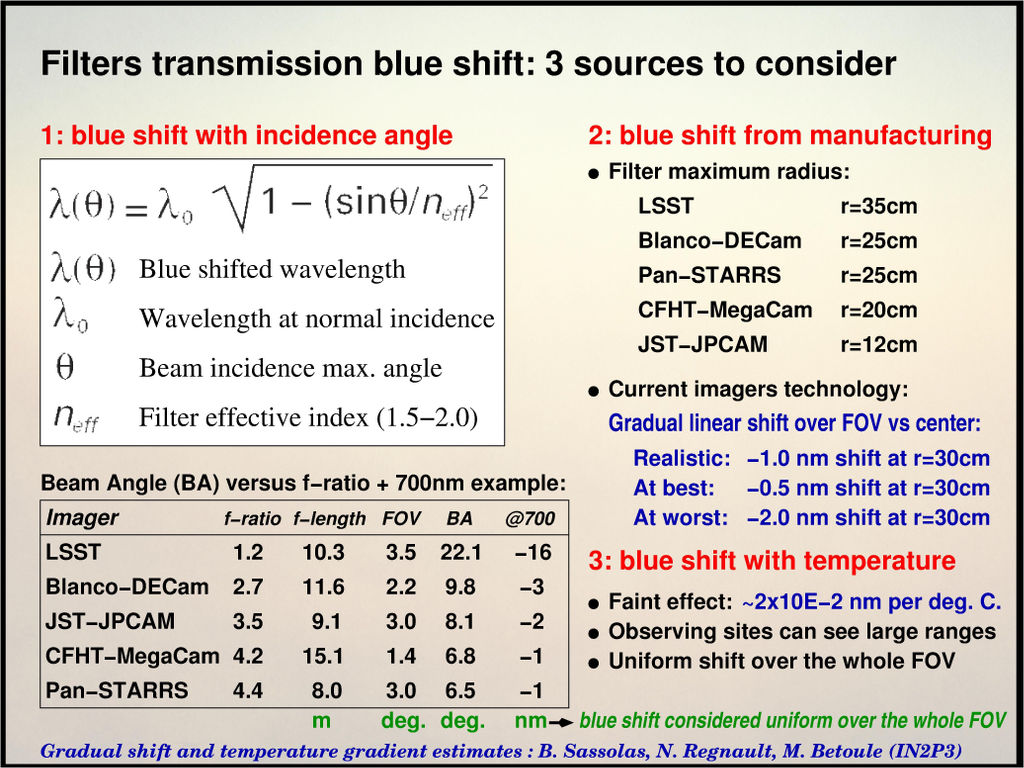
\includegraphics{/Users/coupon/projects/euclid/varTrans/doc/MegaCam/FiltersTransmissionVariabilitySources.XGA.jpg}
\caption{Blue shift in modern filters (from J.-C. Cuillandre)}
\end{figure}

\textbf{{[}Jean{]} I am confused by the impact of the incidence angle on
the filter. If it's really constant, it's less problematic for photo-z's
as the calibration fields will be observed with the same filter. If it
varies across the focal plane, it is an effect we need to study.
However, since the effect is equivalent to a shift caused by
manufacturing, our tests will capture anyway the effect of a shift (due
to either effect), which is fine for this study.}

    \hypertarget{the-sloan-camera}{%
\subsubsection{The Sloan camera}\label{the-sloan-camera}}

From Doi et al. (2010).


    \begin{center}
    \adjustimage{max size={0.9\linewidth}{0.9\paperheight}}{VariableTransmissions_files/VariableTransmissions_15_0.pdf}
    \end{center}
    { \hspace*{\fill} \\}
    
    \begin{center}
    \adjustimage{max size={0.9\linewidth}{0.9\paperheight}}{VariableTransmissions_files/VariableTransmissions_15_1.pdf}
    \end{center}
    { \hspace*{\fill} \\}
    
    \hypertarget{decam-at-the-blanco-telescope}{%
\subsubsection{DECam at the Blanco
telescope}\label{decam-at-the-blanco-telescope}}

Burke et al. (2017) Li et al. (2016)


    \begin{center}
    \adjustimage{max size={0.9\linewidth}{0.9\paperheight}}{VariableTransmissions_files/VariableTransmissions_17_0.pdf}
    \end{center}
    { \hspace*{\fill} \\}
    
    \begin{center}
    \adjustimage{max size={0.9\linewidth}{0.9\paperheight}}{VariableTransmissions_files/VariableTransmissions_17_1.pdf}
    \end{center}
    { \hspace*{\fill} \\}
    
    \hypertarget{hyper-suprime-cam-at-subaru}{%
\subsubsection{Hyper Suprime Cam at
Subaru}\label{hyper-suprime-cam-at-subaru}}

The first \(i\)-band and \(r\)-band filters of the Hyper Suprime Cam
suffered from an important wavelength shift on the cut-on and cut-off
wavelengths in the form of a concentric ring located about half way
between the center and the edge. Miyazaki et al. (2017) report a shift
of up to 7 nm (70 Angstroms). Since 2016, both filters have been
replaced with more uniform transmissions.

\hypertarget{modeling-the-variations}{%
\subsection{Modeling the variations}\label{modeling-the-variations}}

We model in this section the typical filter transmission variations and
a range of amplitudes. Our approach is to be as close to the reality as
possible but with no actual prediction for the typical variations that
the Euclid survey will encounter. The goal is to establish a set of
possible variations and test the impact on photo-\(z\)'s. It must be
used as a ruler to predict the true impact on Euclid (and the actions to
take to address the problem) when the actual variations are known.

Therefore, we will test each effect independently and adopt a range of
amplitudes to mimic what's observed in different cases.

Based on the discussions with people involved in several surveys and the
results presented above, we propose three separate kinds of variations:

\begin{itemize}
\tightlist
\item
  a shift in wavelength (mostly towards the blue)
\item
  a widening (or shortening) of the transmission width
\item
  and a change in slope as a function of wavelength
\end{itemize}

In fact the change in overall sensitivity can also induce a shift in
color if the calibration is unable to correct for it, but this effect is
most probably a second-order effect and we focus primarily on the above
three effects.

As the reference transmission, we model a \(r\)-band filter whose
response is a top-hat function between 5600 and 7000 Angstroms centered
on \(<\lambda>=6300\) Angstroms. The maximum transmission is 0.8.

\hypertarget{shift}{%
\subsubsection{Shift}\label{shift}}

We model the shift by simply shifting the transmission towards the blue
and the red from -100 Angstrom to +100 Angstrom. We see below that the
only impact on the stats compared to the reference filter is a
difference in mean wavelength.

\hypertarget{widening}{%
\subsubsection{Widening}\label{widening}}

We study the impact of a change in standard deviation between -15 and
+15 Angstroms.

\hypertarget{skewing}{%
\subsubsection{Skewing}\label{skewing}}

We model the skewing of the transmission with a linear function with
different slopes whose value at the transmission center is always 0.8.
We vary the slope between \(-1.e-2\times6300\sim-60^{\circ}\) and
\(+1.e-2\times6300\sim60^{\circ}\), which seem to reproduce well the
change in asymetry seen with MegaCam.

\hypertarget{softening}{%
\subsubsection{Softening}\label{softening}}

Finally, we add a fourth kind of variation to take into account the
arbitrary combination of transmissions with different shapes. This can
typically occur when several exposures are stacked together. In addition
to the other effects mentioned above, this will result into a softening
of the transmission edges, which we model by changing the slopes of the
red and blue edges of the transmission.



    \begin{center}
    \adjustimage{max size={0.9\linewidth}{0.9\paperheight}}{VariableTransmissions_files/VariableTransmissions_20_0.pdf}
    \end{center}
    { \hspace*{\fill} \\}
    
    \begin{center}
    \adjustimage{max size={0.9\linewidth}{0.9\paperheight}}{VariableTransmissions_files/VariableTransmissions_20_1.pdf}
    \end{center}
    { \hspace*{\fill} \\}
    
    \begin{center}
    \adjustimage{max size={0.9\linewidth}{0.9\paperheight}}{VariableTransmissions_files/VariableTransmissions_20_2.pdf}
    \end{center}
    { \hspace*{\fill} \\}
    
    \begin{center}
    \adjustimage{max size={0.9\linewidth}{0.9\paperheight}}{VariableTransmissions_files/VariableTransmissions_20_3.pdf}
    \end{center}
    { \hspace*{\fill} \\}
    
    \hypertarget{simulations}{%
\section{Simulations}\label{simulations}}

In this section we perfom the simulations to test the impact of filter
varations on photo-\(z\)'s. The basic principle is to simulate the
fluxes with varying transmissions but compute the photo-\(z\)'s with a
reference filter set.

\hypertarget{the-reference-filter-set}{%
\subsection{The reference filter set}\label{the-reference-filter-set}}

The reference filter set is composed of the Euclid-survey filters,
i.e.~the PLM vis and near-IR filters and the ground-based filters. For
the latter we assume MegaCam-type filters, except for the \(r\)-band
filter for which we assume a transmission whose response is a top-hat
function between 5600 and 7000 Angstroms centered on =6300 Angstroms, as
we adopted in the previous section, with the slight difference that the
maximum transmission is 0.5 (as opposed to 0.8), to mimic the
attenuation from the atmosphere and the mirror.



    \begin{center}
    \adjustimage{max size={0.9\linewidth}{0.9\paperheight}}{VariableTransmissions_files/VariableTransmissions_22_1.pdf}
    \end{center}
    { \hspace*{\fill} \\}
    
    \hypertarget{the-variable-filter-set}{%
\subsection{The variable filter set}\label{the-variable-filter-set}}

We limit ourselves to the variations of the \(r\)-band filter and focus
on the photo-\(z\) mean redshift in the interval where the Balmer break
goes through the filter wavelength range, i.e between \(0.3<z<0.8\). We
expect that similar trends will occur at different redshifts when other
filters are affected by variable transmissions, but we have no reason to
think that the effect will be any weaker for the \(r\)-band than for the
other bands, even when accounting for the stretch of the SED with
redshift (that could potentielly increase the effect in redder bands),
as the performances are always divided by a factor 1+\(z\).

The variations we adopt are identical to those described above and are
composed of 10 shifts between -100 and +100 Angstroms, 10 widenings
between -20 and +20 Angstroms, 10 angles for the skewing, and 10
softening between 0 and 100 angstroms.


    \hypertarget{the-simulated-sample}{%
\subsection{The simulated sample}\label{the-simulated-sample}}

We start from real galaxies from the COSMOS field (``COSMOS2015'',
Laigle et al.~2016) for which a spectral energy distribution (SED) has
been fitted to each of them (using the available 30 photometric bands
and the best photo-\(z\) estimate, Ilbert et al.) and we emulate the
galaxies' fluxes in the fixed set of transmissions, as well as the
additional 30 variable \(r\)-band transmission's fluxes.

The main sample is split into two equal samples along a constant RA line
to ensure their independence: a deeper calibration sample (``calib'')
and a target sample (``valid'') at the Euclid-Wide depth.




    The errors are computed assuming the depth requirements from the Euclid
COG group (J.-C. Cuillandre, private communication). Those were also
adopted for the photo-\(z\) data chalenge 3 (DC3, see documentation).
The flux error includes both the Poisson noise from the object
brightness and the sky background. The 10-sigmas depths
(background-dominated) in optimal apertures
(\(1.7*{{\rm FWHM}_{\rm PSF}}^{0.5}\)) are given below:

\begin{longtable}[]{@{}lc@{}}
\toprule
Filter & Depths (10 sigmas)\tabularnewline
\midrule
\endhead
\(u\) & 23.6\tabularnewline
\(g\) & 24.5\tabularnewline
\(r\) & 23.9\tabularnewline
\(i\) & 23.6\tabularnewline
\(z\) & 23.4\tabularnewline
vis & 24.6\tabularnewline
\(Y\) & 23.0\tabularnewline
\(J\) & 23.0\tabularnewline
\(H\) & 23.0\tabularnewline
\bottomrule
\end{longtable}

The calibration sample has depths 5 times that of the target catalogue
(= 25 times the observing time).

Full details are given in the data challenge 3 documentation.




    \hypertarget{the-simulations}{%
\subsection{The simulations}\label{the-simulations}}

\hypertarget{adopted-metric}{%
\subsubsection{Adopted metric}\label{adopted-metric}}

The photo-\(z\) pipeline, developed by the OU-PHZ and the SDC-CH, will
proceed in two main steps to compute the photo-\(z\) PDFs. The first
step consists in producing a PDF for each individual galaxy with the
adaquate algorithm to meet the precision requirement (i.e.~on
photo-\(z\) scatter and outlier fraction).

The second step consists in correcting for the mean redshift bias to
meet the accuracy requirement, but done for an ensemble of galaxies or
directly per redshift bin. In fact several strategies are explored,
including a correction per color bin (instead of the full redshift bin),
but the result should always be that the mean redshift bias \emph{per
bin} must be zero after correction. The operation will most probably be
performed using a set of reference spectroscopic redshifts properly
weighted to represent the full population, followed by a validation
phase involving cluster-\(z\)'s.

The redshift bins are built using a redshift point estimate extracted
from the PDF or (but a simple color selection is also possible), and the
mean redshift per bin is computed as the mean of the stacked PDFs.

Our metric to measure the impact of variable filters on photo-\(z\)'s is
the systematic shift \(\Delta z_\mathrm{var}\) affecting the PDF in a
given redshift bin, compared to the mean redshift measured when the
transmissions are fixed (i.e.~when both the calibration and target
samples share the exact same filter set):

    \begin{equation}
\Delta \langle z \rangle _\mathrm{var} = \langle z \rangle_\mathrm{var}- \langle z \rangle_\mathrm{fix}
\end{equation}

    \hypertarget{the-photo-z-algorithm}{%
\subsubsection{\texorpdfstring{The photo-\(z\)
algorithm}{The photo-z algorithm}}\label{the-photo-z-algorithm}}

We use the NNPZ algorithm to compute the photo-\(z\) PDFs (see details
in Tanaka et al.~2017, PASJ, psx077, with the exception that here we do
not make use of any flux, only colors in the form of magnitude
differences), which is the current baseline for the OU-PHZ pipeline.
This algorithm has given one of the best performances during the PHZ
data challenge 2 and is best mastered by the author of this note, but
any other algorithm meeting the requirements on precision could be used
without affecting the conclusions of this report.

We extract the median of each PDF as the corresponding point estimate,
used for defining the redshift bins and deriving the basic photo-\(z\)
statistics (scatter and outlier fraction).

\hypertarget{procedure}{%
\subsubsection{Procedure}\label{procedure}}

We first compute the photo-\(z\)'s using the exact same set of fixed
transmissions for both the calibration and target samples. This step
serves as a reference for the various photo-\(z\) performance
statistics.

Secondly, we change the transmission and emulate new fluxes for the
target sample. However, we estimate again the photo-\(z\) using the
identical calibration sample as before, whose fluxes were computed with
the fixed set of transmission (i.e.~only the fluxes have changed, not
the way we compute the photo-\(z\)'s). This methodology is equivalent to
ignoring the variability of the transmissions when computing the
photometric redshifts. For SED fitting method, this would be equivalent
to always using the fixed transmissions when computing the flux grid,
but applied to galaxies whose fluxes are computed with variable
transmissions.

Lastly, we measure the mean redshift per redshift bin, both in the case
of fixed transmissions and in the case of variable transmissions. We
record the difference between the two and we repeat the procedure for
all the different type of variations described above.


    \hypertarget{results}{%
\section{Results}\label{results}}

\hypertarget{photo-z-performances-for-the-fixed-transmissions}{%
\subsection{\texorpdfstring{Photo-\(z\) performances for the fixed
transmissions}{Photo-z performances for the fixed transmissions}}\label{photo-z-performances-for-the-fixed-transmissions}}

We first show the photo-\(z\) performances in the fixed transmission
case (when both calibration and target sample fluxes are computed in the
fixed filter set).

\hypertarget{scatter-plot}{%
\subsubsection{Scatter plot}\label{scatter-plot}}

Below is the photo-\(z\) (\(z_\mathrm{median}\) estimates) versus the
true redshift.


    \begin{center}
    \adjustimage{max size={0.9\linewidth}{0.9\paperheight}}{VariableTransmissions_files/VariableTransmissions_37_0.pdf}
    \end{center}
    { \hspace*{\fill} \\}
    
    \begin{center}
    \adjustimage{max size={0.9\linewidth}{0.9\paperheight}}{VariableTransmissions_files/VariableTransmissions_37_1.pdf}
    \end{center}
    { \hspace*{\fill} \\}
    
    The top figure shows the comparison for the full galaxy sample (i.e.~all
redshifts) cut at vis\(<24.5\). The bottom figure shows the comparison
with a additional cut in redshift \(0.2<z<2.0\) corresponding to the
limits of the shear sample.

The statistics shown in the figures are computed on the ``spec-\(z\)''
sample (the subset matching the real galaxies having a spec-\(z\)) using
the weights calculated to represent the full population and given a cut
at \(\mathrm{vis}<24.5\), SNR\(>10\) and \(0.2<z<2.0\) to match the
shear sample. They are expressed for the point estimates (the median
redshift of the PDFs) and slightly differ from the metric defined by
OU-PHZ which are based on the stacked PDFs. Nevertheless, these
statistics suggest the photo-\(z\)'s meet the requirements
(\(\sigma < 0.05\times(1+z)\) and \(\eta < 10\%\)) and are therefore
well suited for our tests.

\hypertarget{mean-redshift}{%
\subsubsection{Mean redshift}\label{mean-redshift}}

In the example below we show the stacked PDFs in the redshift interval
\(0.5<z<0.6\).

Starting from now and for the rest of the note, galaxies are no longer
weighted. This is to avoid the dispersion caused by the weighting scheme
when splitting per redshift bins. This point will be addressed later, by
running the simulations on the full sample.


    

    
    
    \begin{verbatim}
<matplotlib.text.Text at 0x1a0fe4b8d0>
    \end{verbatim}

    

    \begin{center}
    \adjustimage{max size={0.9\linewidth}{0.9\paperheight}}{VariableTransmissions_files/VariableTransmissions_39_1.pdf}
    \end{center}
    { \hspace*{\fill} \\}
    
    The left-hand plot shows the redshift distribution for the true
redhsifts (histogram of the point estimates), in red, and the sum of the
estimated PDFs in blue.

The right-hand panel shows the stacked PDF shifted with respect to the
true value. The various statistics correspond the metric define by
OU-PHZ for measuring the photo-z performances on PDFs.

The mean redshift bias is shown as the \(\Delta z\) value.

\hypertarget{photo-z-performances-for-the-variable-transmissions}{%
\subsection{\texorpdfstring{Photo-\(z\) performances for the variable
transmissions}{Photo-z performances for the variable transmissions}}\label{photo-z-performances-for-the-variable-transmissions}}

In this section we compare the fixed-transmission quantities versus
those computed with the variable transmissions.

\hypertarget{flux-differences}{%
\subsubsection{Flux differences}\label{flux-differences}}

We first show the difference in magnitudes caused by the variable
transmissions as a function of redshift. For this we compare the
\(r\)-band fluxes computed in the variable transmissions in the three
most extreme cases (shifted by -100 Angstroms, widened by 20 Angstrom
and a slope of -0.63), compared to the \(r\)-band fluxes computed in the
fixed transmission.


    \begin{center}
    \adjustimage{max size={0.9\linewidth}{0.9\paperheight}}{VariableTransmissions_files/VariableTransmissions_41_0.pdf}
    \end{center}
    { \hspace*{\fill} \\}
    
    \begin{center}
    \adjustimage{max size={0.9\linewidth}{0.9\paperheight}}{VariableTransmissions_files/VariableTransmissions_41_1.pdf}
    \end{center}
    { \hspace*{\fill} \\}
    
    \begin{center}
    \adjustimage{max size={0.9\linewidth}{0.9\paperheight}}{VariableTransmissions_files/VariableTransmissions_41_2.pdf}
    \end{center}
    { \hspace*{\fill} \\}
    
    \begin{center}
    \adjustimage{max size={0.9\linewidth}{0.9\paperheight}}{VariableTransmissions_files/VariableTransmissions_41_3.pdf}
    \end{center}
    { \hspace*{\fill} \\}
    
    As expected, we see that the redshift range where the Balmer break goes
through the \(r\)-band, i.e. \(0.3<z<0.8\), is the most affected. The
shift, due to our chosen range (-100 to +100 Angstroms) is the most
problematic case, leading up to 0.1 magnitude difference at worst
(\(z\sim0.5\)). The widening has, on average, almost no impact, but this
is also expected since in this experiment we neglect the calibration
issues caused by the variable transmissions. The widening will most
ptrobably cause, however, addional scattering, but this is barely
distinguishable from the statistical scatter in this figure.

Interestingly, the change in slope seems to create a systematic shift
similar to the shift in wavelength. This confirms what we saw previously
when computing the moments of the transmission: the change in slope is
causing a shift of the mean wavelength of the transmission.

\hypertarget{scatter-plot}{%
\subsubsection{Scatter plot}\label{scatter-plot}}

We show the median redshift estimate versus the true redshift for the
fixed-transmission case (left) and the variable-transmission case
(right), here a shift of -100 Angstroms.


    \begin{center}
    \adjustimage{max size={0.9\linewidth}{0.9\paperheight}}{VariableTransmissions_files/VariableTransmissions_43_0.pdf}
    \end{center}
    { \hspace*{\fill} \\}
    
    The shift in the transmission causes a systematic shift in the redshift.
The target fluxes are affected by a blue shift (-100 Angstroms), causing
an artificial red shift of the SEDs, which explains why the true
redshift is shifted towards lower values.

\hypertarget{mean-redshift}{%
\subsubsection{Mean redshift}\label{mean-redshift}}

The figure below shows the stacked PDF in the variable transmission
case.


    

    
    
    \begin{verbatim}
<matplotlib.text.Text at 0x1a10435910>
    \end{verbatim}

    

    \begin{center}
    \adjustimage{max size={0.9\linewidth}{0.9\paperheight}}{VariableTransmissions_files/VariableTransmissions_45_1.pdf}
    \end{center}
    { \hspace*{\fill} \\}
    
    Similarly to the scatter plot, a clear systematic mean redshift shift is
seen, both for the redshift distribution and the stacked PDFs.

In the next figures we show \(\Delta z_\mathrm{var}\) as a function of
redshift, for the shift, the widening and the skewing of the
transmission. In each case we only show the two extreme cases as well as
the middle case which corresponds as the smallest variation.



    \begin{center}
    \adjustimage{max size={0.9\linewidth}{0.9\paperheight}}{VariableTransmissions_files/VariableTransmissions_48_0.pdf}
    \end{center}
    { \hspace*{\fill} \\}
    


    \begin{center}
    \adjustimage{max size={0.9\linewidth}{0.9\paperheight}}{VariableTransmissions_files/VariableTransmissions_50_0.pdf}
    \end{center}
    { \hspace*{\fill} \\}
    
    \begin{center}
    \adjustimage{max size={0.9\linewidth}{0.9\paperheight}}{VariableTransmissions_files/VariableTransmissions_50_1.pdf}
    \end{center}
    { \hspace*{\fill} \\}
    
    \begin{center}
    \adjustimage{max size={0.9\linewidth}{0.9\paperheight}}{VariableTransmissions_files/VariableTransmissions_50_2.pdf}
    \end{center}
    { \hspace*{\fill} \\}
    
    \begin{center}
    \adjustimage{max size={0.9\linewidth}{0.9\paperheight}}{VariableTransmissions_files/VariableTransmissions_50_3.pdf}
    \end{center}
    { \hspace*{\fill} \\}
    
    The results above confirm the trends observed in provious sections, and
we can already conclude that the shift is the most problematic issue,
whereas the impact from widening and the skewing remains lower. As
stated above the effect from the skewing shows a similar behaviour as
the shift.

Finally we focus on the redshift range that is most impacted,
\(0.55 < z < 0.7\) and we show \(\Delta z_\mathrm{var}\) as a function
of the different simulated variations.


    \begin{center}
    \adjustimage{max size={0.9\linewidth}{0.9\paperheight}}{VariableTransmissions_files/VariableTransmissions_52_0.pdf}
    \end{center}
    { \hspace*{\fill} \\}
    
    \begin{center}
    \adjustimage{max size={0.9\linewidth}{0.9\paperheight}}{VariableTransmissions_files/VariableTransmissions_52_1.pdf}
    \end{center}
    { \hspace*{\fill} \\}
    
    \begin{center}
    \adjustimage{max size={0.9\linewidth}{0.9\paperheight}}{VariableTransmissions_files/VariableTransmissions_52_2.pdf}
    \end{center}
    { \hspace*{\fill} \\}
    
    \begin{center}
    \adjustimage{max size={0.9\linewidth}{0.9\paperheight}}{VariableTransmissions_files/VariableTransmissions_52_3.pdf}
    \end{center}
    { \hspace*{\fill} \\}
    
    The first figure above shows the linear dependence of the redshift bias
as a function of the transmission shift. We overplotted the theoretical
prediction assuming that the shift can be directly interpreted as an
additional redshift on average. The two curves show very similar
behaviour which confirms that a shift in wavelength can be directly
translated into a redshift bias.

    \hypertarget{conclusions}{%
\section{Conclusions}\label{conclusions}}

We have tested the impact of variable transmissions on photo-\(z\)'s
using simulated fluxes based on the best-fit templates of real galaxies
observed with 30 photometric bands in the COSMOS field, and whose
emulated fluxes were perturbed according to the minimum-flux SNRs
required to meet the precision requirements on photo-\(z\) in Euclid.

We only modelled the variations on the \(r\)-band and we measured the
impact in the redshift range which is the most affected, \(0.3<z<0.8\),
due to the predominance of the Balmer break (4000 Angstroms) to
constraint the photometric redshift in this interval.

We modeled three main typical variations: a shift in wavelength, a
centered widening (or shortening) of the bandpass and a skewing of the
transmission, calibrated using real variations measured on various
bandpasses and communicated by OU-EXT, the COG, or found in the
literature.

The main impact is found to be on the mean redshift of an ensemble of
galaxies (the so-called mean redshift bias), and our main findings can
be summarized as follow:

\begin{itemize}
\item
  The most problematic effect is a systematic shift in mean redshift and
  is due to the shift in wavelength of the transmission. The impact on
  the mean redshift scales linearly with the inverse of the shift in
  wavelength for the galaxies whose Balmer break is passing through the
  transmission. For example a typical shift of +40 Angstroms in the
  \(r\)-band will cause a mean redshift bias equal to -40/4000.0 =
  -0.01, i.e.~about three times the requirement.
\item
  consequently, a shift as small as 12 Angstrom (1.2 nm) is on the same
  order as the requirement on the bias
\item
  after calibration, the widening of the transmission has no impact on
  the mean redshift
\item
  the main effect of the skewing of the transmission is to increase the
  transmission mean wavelength, hence it has the same affect as a shift
  of the transmission
\item
  overall the simulations show that the mean wavelength of the filter is
  the main quantity that impacts the mean redshift for an ensemble of
  galaxies
\item
  it also means that simply recording the mean wavelength of the
  transmission and shifting it accordingly seems to be sufficient to
  correct for the bias
\end{itemize}

So, it is clear that filter variations impact the mean redshift of large
samples of galaxies, even when the variation is small. However, it seems
not necessary to propagate the full transmission for each object, but
only the mean wavelength of the transmission to correct for the effect.


    % Add a bibliography block to the postdoc
    
    
    
    \end{document}
